% ============================================================
% NIFTY 100 Cross-Sectional Forecasting Architecture Diagram
% Compile with: pdflatex architecture_tikz.tex
% ============================================================
\documentclass[border=10pt]{standalone}
\usepackage[utf8]{inputenc}
\usepackage{tikz}
\usetikzlibrary{
  positioning,
  shapes.geometric,
  arrows.meta,
  fit,
  backgrounds,
  calc,
  decorations.pathreplacing
}

\definecolor{datablue}{HTML}{3B82F6}
\definecolor{datalightblue}{HTML}{DBEAFE}
\definecolor{prepgreen}{HTML}{22C55E}
\definecolor{preplightgreen}{HTML}{DCFCE7}
\definecolor{modelorange}{HTML}{F97316}
\definecolor{modellightorange}{HTML}{FFEDD5}
\definecolor{evalpurple}{HTML}{A855F7}
\definecolor{evallightpurple}{HTML}{F3E8FF}
\definecolor{trainred}{HTML}{EF4444}
\definecolor{trainlightred}{HTML}{FEE2E2}
\definecolor{arrowgray}{HTML}{6B7280}

\begin{document}
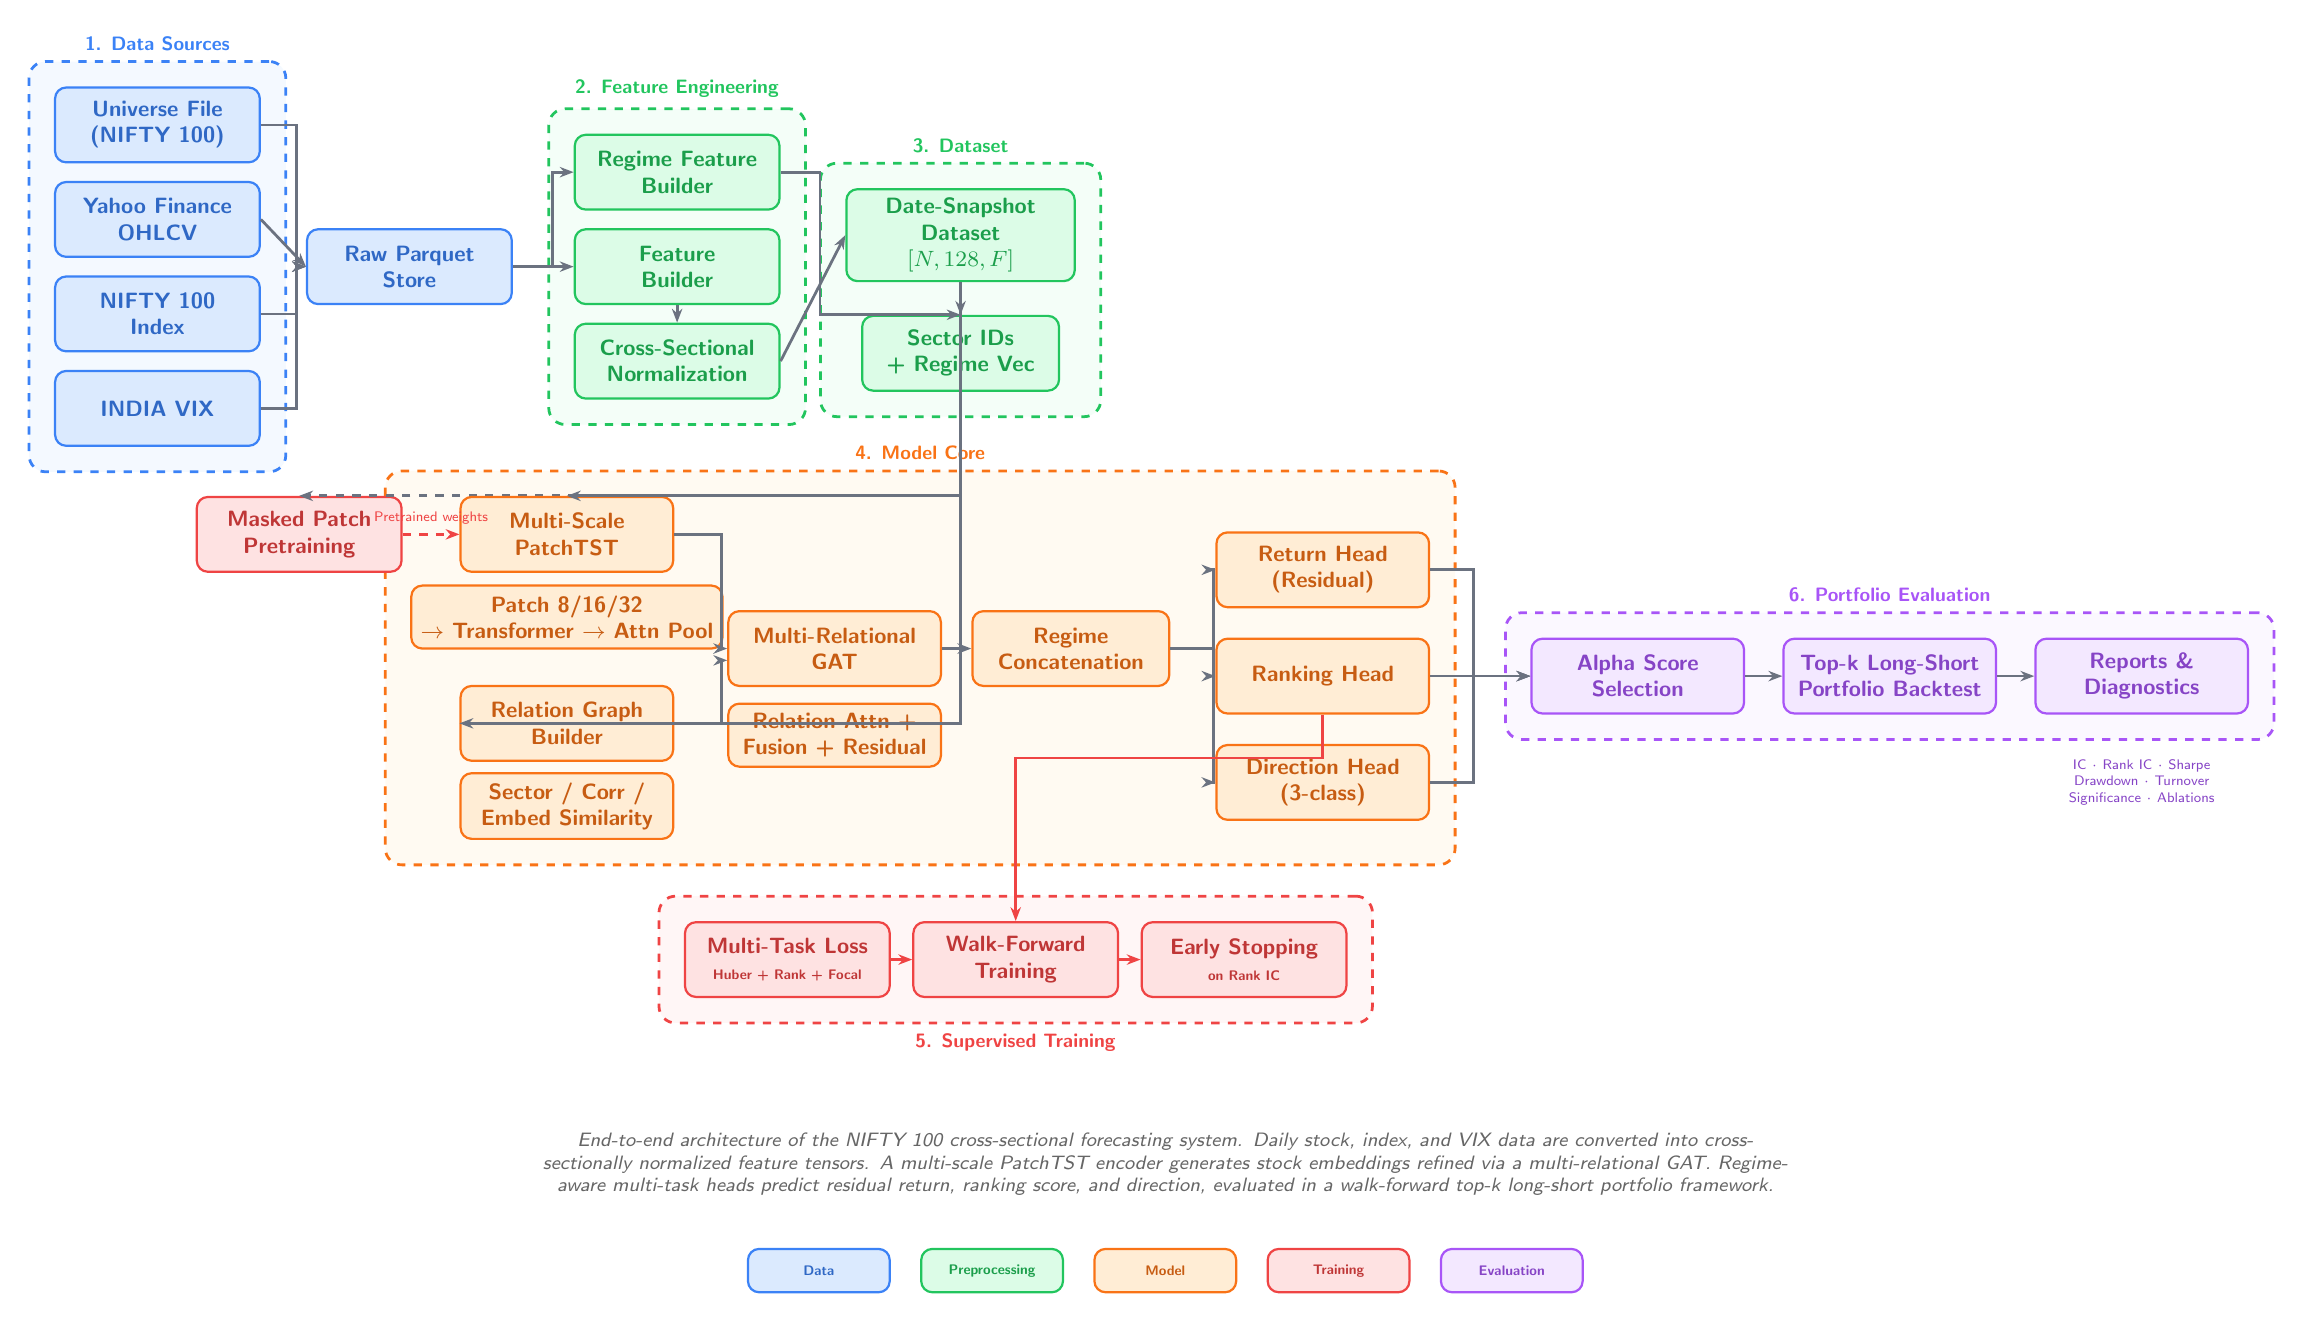
\begin{tikzpicture}[
  >=Stealth,
  every node/.style={font=\sffamily\small},
  databox/.style={rectangle, rounded corners=4pt, draw=datablue, fill=datalightblue,
    minimum width=2.6cm, minimum height=0.95cm, align=center,
    text=datablue!80!black, font=\sffamily\footnotesize\bfseries, line width=0.8pt},
  prepbox/.style={rectangle, rounded corners=4pt, draw=prepgreen, fill=preplightgreen,
    minimum width=2.6cm, minimum height=0.95cm, align=center,
    text=prepgreen!80!black, font=\sffamily\footnotesize\bfseries, line width=0.8pt},
  modelbox/.style={rectangle, rounded corners=4pt, draw=modelorange, fill=modellightorange,
    minimum width=2.7cm, minimum height=0.95cm, align=center,
    text=modelorange!80!black, font=\sffamily\footnotesize\bfseries, line width=0.8pt},
  trainbox/.style={rectangle, rounded corners=4pt, draw=trainred, fill=trainlightred,
    minimum width=2.6cm, minimum height=0.95cm, align=center,
    text=trainred!80!black, font=\sffamily\footnotesize\bfseries, line width=0.8pt},
  evalbox/.style={rectangle, rounded corners=4pt, draw=evalpurple, fill=evallightpurple,
    minimum width=2.7cm, minimum height=0.95cm, align=center,
    text=evalpurple!80!black, font=\sffamily\footnotesize\bfseries, line width=0.8pt},
  detail/.style={font=\sffamily\tiny\bfseries},
  groupdata/.style={rectangle, rounded corners=6pt, draw=datablue, dashed, line width=1pt, fill=datalightblue!30, inner sep=9pt},
  groupprep/.style={rectangle, rounded corners=6pt, draw=prepgreen, dashed, line width=1pt, fill=preplightgreen!30, inner sep=9pt},
  groupmodel/.style={rectangle, rounded corners=6pt, draw=modelorange, dashed, line width=1pt, fill=modellightorange!30, inner sep=9pt},
  grouptrain/.style={rectangle, rounded corners=6pt, draw=trainred, dashed, line width=1pt, fill=trainlightred!30, inner sep=9pt},
  groupeval/.style={rectangle, rounded corners=6pt, draw=evalpurple, dashed, line width=1pt, fill=evallightpurple!30, inner sep=9pt},
  myarrow/.style={-{Stealth[length=5pt]}, line width=1pt, color=arrowgray},
  grouplabel/.style={font=\sffamily\scriptsize\bfseries, text=black!70}
]

% Top row: stages 1-3
\node[databox] (universe) at (0,5.1) {Universe File\\(NIFTY 100)};
\node[databox] (yahoo) at (0,3.9) {Yahoo Finance\\OHLCV};
\node[databox] (niftyidx) at (0,2.7) {NIFTY 100\\Index};
\node[databox] (vix) at (0,1.5) {INDIA VIX};
\node[databox] (rawstore) at (3.2,3.3) {Raw Parquet\\Store};

\draw[myarrow] (universe.east) -- ++(0.45,0) |- (rawstore.west);
\draw[myarrow] (yahoo.east) -- (rawstore.west);
\draw[myarrow] (niftyidx.east) -- ++(0.45,0) |- (rawstore.west);
\draw[myarrow] (vix.east) -- ++(0.45,0) |- (rawstore.west);

\begin{scope}[on background layer]
  \node[groupdata, fit=(universe)(yahoo)(niftyidx)(vix),
    label={[grouplabel,text=datablue]above:{\textbf{1. Data Sources}}}] (g1) {};
\end{scope}

% Stage 2: features
\node[prepbox] (regime) at (6.6,4.5) {Regime Feature\\Builder};
\node[prepbox] (feateng) at (6.6,3.3) {Feature\\Builder};
\node[prepbox] (xsnorm) at (6.6,2.1) {Cross-Sectional\\Normalization};

\draw[myarrow] (rawstore.east) -- (feateng.west);
\draw[myarrow] (rawstore.east) -- ++(0.5,0) |- (regime.west);
\draw[myarrow] (feateng) -- (xsnorm);

\begin{scope}[on background layer]
  \node[groupprep, fit=(regime)(feateng)(xsnorm),
    label={[grouplabel,text=prepgreen]above:{\textbf{2. Feature Engineering}}}] (g2) {};
\end{scope}

% Stage 3: dataset
\node[prepbox, minimum width=2.9cm] (dataset) at (10.2,3.7) {Date-Snapshot\\Dataset\\\footnotesize$[N,128,F]$};
\node[prepbox, minimum width=2.5cm] (sectorids) at (10.2,2.2) {Sector IDs\\+ Regime Vec};

\draw[myarrow] (xsnorm.east) -- (dataset.west);
\draw[myarrow] (dataset.south) -- (sectorids.north);
\draw[myarrow] (regime.east) -- ++(0.5,0) |- (sectorids.north);

\begin{scope}[on background layer]
  \node[groupprep, fit=(dataset)(sectorids),
    label={[grouplabel,text=prepgreen]above:{\textbf{3. Dataset}}}] (g3) {};
\end{scope}

% Bottom row: stages 4-6
\node[trainbox] (pretrain) at (1.8,-0.1) {Masked Patch\\Pretraining};
\draw[myarrow, dashed, color=arrowgray] (dataset.south) |- (pretrain.north);

% Stage 4: model core
\node[modelbox] (patchtst) at (5.2,-0.1) {Multi-Scale\\PatchTST};
\node[modelbox, minimum height=0.8cm] (patchdetail) at (5.2,-1.15) {Patch 8/16/32\\$\rightarrow$ Transformer $\rightarrow$ Attn Pool};
\node[modelbox] (graphbuild) at (5.2,-2.5) {Relation Graph\\Builder};
\node[modelbox, minimum height=0.8cm] (graphdetail) at (5.2,-3.55) {Sector / Corr /\\Embed Similarity};

\node[modelbox] (gat) at (8.6,-1.55) {Multi-Relational\\GAT};
\node[modelbox, minimum height=0.8cm] (gatdetail) at (8.6,-2.65) {Relation Attn +\\Fusion + Residual};
\node[modelbox, minimum width=2.5cm] (regimecat) at (11.6,-1.55) {Regime\\Concatenation};

\node[modelbox] (headret) at (14.8,-0.55) {Return Head\\(Residual)};
\node[modelbox] (headrank) at (14.8,-1.9) {Ranking Head};
\node[modelbox] (headdir) at (14.8,-3.25) {Direction Head\\(3-class)};

\draw[myarrow] (dataset.south) |- (patchtst.north);
\draw[myarrow] (sectorids.south) |- (graphbuild.west);
\draw[myarrow] (patchtst.east) -- ++(0.6,0) |- (gat.west);
\draw[myarrow] (graphbuild.east) -- ++(0.6,0) |- ($(gat.west)+(0,-0.15)$);
\draw[myarrow, dashed, color=trainred] (pretrain.east) -- node[above, font=\sffamily\tiny, text=trainred] {Pretrained weights} (patchtst.west);
\draw[myarrow] (gat.east) -- (regimecat.west);
\draw[myarrow] (regimecat.east) -- ++(0.55,0) |- (headret.west);
\draw[myarrow] (regimecat.east) -- ++(0.55,0) |- (headrank.west);
\draw[myarrow] (regimecat.east) -- ++(0.55,0) |- (headdir.west);

\begin{scope}[on background layer]
  \node[groupmodel, fit=(patchtst)(patchdetail)(graphbuild)(graphdetail)(gat)(gatdetail)(regimecat)(headret)(headrank)(headdir),
    label={[grouplabel,text=modelorange]above:{\textbf{4. Model Core}}}] (g4) {};
\end{scope}

% Stage 5: supervised training
\node[trainbox] (mtloss) at (8.0,-5.5) {Multi-Task Loss\\{\tiny Huber + Rank + Focal}};
\node[trainbox] (walkfwd) at (10.9,-5.5) {Walk-Forward\\Training};
\node[trainbox] (earlystop) at (13.8,-5.5) {Early Stopping\\{\tiny on Rank IC}};

\draw[myarrow, color=trainred] (headrank.south) -- ++(0,-0.55) -| (walkfwd.north);
\draw[myarrow, color=trainred] (mtloss.east) -- (walkfwd.west);
\draw[myarrow, color=trainred] (walkfwd.east) -- (earlystop.west);

\begin{scope}[on background layer]
  \node[grouptrain, fit=(mtloss)(walkfwd)(earlystop),
    label={[grouplabel,text=trainred]below:{\textbf{5. Supervised Training}}}] (g5) {};
\end{scope}

% Stage 6: evaluation
\node[evalbox] (alphasel) at (18.8,-1.9) {Alpha Score\\Selection};
\node[evalbox] (portfolio) at (22.0,-1.9) {Top-k Long-Short\\Portfolio Backtest};
\node[evalbox] (reports) at (25.2,-1.9) {Reports \&\\Diagnostics};

\draw[myarrow] (headret.east) -- ++(0.55,0) |- (alphasel.west);
\draw[myarrow] (headrank.east) -- ++(0.55,0) -- (alphasel.west);
\draw[myarrow] (headdir.east) -- ++(0.55,0) |- (alphasel.west);
\draw[myarrow] (alphasel.east) -- (portfolio.west);
\draw[myarrow] (portfolio.east) -- (reports.west);

\node[font=\sffamily\tiny, text=evalpurple!80!black, align=center] at (25.2,-3.25)
  {IC $\cdot$ Rank IC $\cdot$ Sharpe\\Drawdown $\cdot$ Turnover\\Significance $\cdot$ Ablations};

\begin{scope}[on background layer]
  \node[groupeval, fit=(alphasel)(portfolio)(reports),
    label={[grouplabel,text=evalpurple]above:{\textbf{6. Portfolio Evaluation}}}] (g6) {};
\end{scope}

% Caption and legend
\node[font=\sffamily\scriptsize, text=black!60, align=center, text width=23cm] at (12.8,-8.1)
  {\textit{End-to-end architecture of the NIFTY 100 cross-sectional forecasting system. Daily stock, index, and VIX data are converted into cross-sectionally normalized feature tensors. A multi-scale PatchTST encoder generates stock embeddings refined via a multi-relational GAT. Regime-aware multi-task heads predict residual return, ranking score, and direction, evaluated in a walk-forward top-k long-short portfolio framework.}};

\node[databox, minimum width=1.8cm, minimum height=0.55cm, font=\sffamily\tiny\bfseries] (leg1) at (8.4,-9.45) {Data};
\node[prepbox, minimum width=1.8cm, minimum height=0.55cm, font=\sffamily\tiny\bfseries] (leg2) at (10.6,-9.45) {Preprocessing};
\node[modelbox, minimum width=1.8cm, minimum height=0.55cm, font=\sffamily\tiny\bfseries] (leg3) at (12.8,-9.45) {Model};
\node[trainbox, minimum width=1.8cm, minimum height=0.55cm, font=\sffamily\tiny\bfseries] (leg4) at (15.0,-9.45) {Training};
\node[evalbox, minimum width=1.8cm, minimum height=0.55cm, font=\sffamily\tiny\bfseries] (leg5) at (17.2,-9.45) {Evaluation};

\end{tikzpicture}
\end{document}
